%% Version 4.3.2, 25 August 2014
%
%%%%%%%%%%%%%%%%%%%%%%%%%%%%%%%%%%%%%%%%%%%%%%%%%%%%%%%%%%%%%%%%%%%%%%
% Template.tex --  LaTeX-based template for submissions to the 
% American Meteorological Society
%
% Template developed by Amy Hendrickson, 2013, TeXnology Inc., 
% amyh@texnology.com, http://www.texnology.com
% following earlier work by Brian Papa, American Meteorological Society
%
% Email questions to latex@ametsoc.org.
%
%%%%%%%%%%%%%%%%%%%%%%%%%%%%%%%%%%%%%%%%%%%%%%%%%%%%%%%%%%%%%%%%%%%%%
% PREAMBLE
%%%%%%%%%%%%%%%%%%%%%%%%%%%%%%%%%%%%%%%%%%%%%%%%%%%%%%%%%%%%%%%%%%%%%

%% Start with one of the following:
% DOUBLE-SPACED VERSION FOR SUBMISSION TO THE AMS
\documentclass{ametsoc}

% TWO-COLUMN JOURNAL PAGE LAYOUT---FOR AUTHOR USE ONLY
% \documentclass[twocol]{ametsoc}

%%%%%%%%%%%%%%%%%%%%%%%%%%%%%%%%
%%% To be entered only if twocol option is used

\journal{jtech}

%  Please choose a journal abbreviation to use above from the following list:
% 
%   jamc     (Journal of Applied Meteorology and Climatology)
%  jtech     (Journal of Atmospheric and Oceanic Technology)
%   jhm      (Journal of Hydrometeorology)
%   jpo     (Journal of Physical Oceanography)
%   jas      (Journal of Atmospheric Sciences)	
%   jcli      (Journal of Climate)
%   mwr      (Monthly Weather Review)
%   wcas      (Weather, Climate, and Society)
%   waf       (Weather and Forecasting)
%   bams (Bulletin of the American Meteorological Society)
%   ei    (Earth Interactions)

%%%%%%%%%%%%%%%%%%%%%%%%%%%%%%%%
%Citations should be of the form ``author year''  not ``author, year''
\bibpunct{(}{)}{;}{a}{}{,}

%%%%%%%%%%%%%%%%%%%%%%%%%%%%%%%%

%%% To be entered by author:

%% May use \\ to break lines in title:

\title{Estimating $\chi$ and $K_T$ from fast-reponse thermistors on traditional shipboard CTDs: sources of uncertainty and bias.}

%%% Enter authors' names, as you see in this example:
%%% Use \correspondingauthor{} and \thanks{Current Affiliation:...}
%%% immediately following the appropriate author.
%%%
%%% Note that the \correspondingauthor{} command is NECESSARY.
%%% The \thanks{} commands are OPTIONAL.

    %\authors{Author One\correspondingauthor{Author One, 
    % American Meteorological Society, 
    % 45 Beacon St., Boston, MA 02108.}
% and Author Two\thanks{Current affiliation: American Meteorological Society, 
    % 45 Beacon St., Boston, MA 02108.}}

\authors{Andy Pickering\correspondingauthor{College of Earth, Ocean, and Atmospheric Sciences, Oregon State University, Corvallis, OR.}}

%% Follow this form:
     \affiliation{College of Earth, Ocean, and Atmospheric Sciences, Oregon State University, Corvallis, OR.}

%\affiliation{}

%% Follow this form:
    %\email{latex@ametsoc.org}

\email{}

%% If appropriate, add additional authors, different affiliations:
    \extraauthor{Jonathan Nash}
    \extraaffil{College of Earth, Ocean, and Atmospheric Sciences, Oregon State University, Corvallis, OR.}

    \extraauthor{Jim Moum}
    \extraaffil{College of Earth, Ocean, and Atmospheric Sciences, Oregon State University, Corvallis, OR.}

    \extraauthor{Jen MacKinnon}
    \extraaffil{UCSD / Scripps Institute of Oceanography}



%\extraauthor{}
%\extraaffil{}

%% May repeat for a additional authors/affiliations:

%\extraauthor{}
%\extraaffil{}

%%%%%%%%%%%%%%%%%%%%%%%%%%%%%%%%%%%%%%%%%%%%%%%%%%%%%%%%%%%%%%%%%%%%%
% ABSTRACT
%
% Enter your abstract here
% Abstracts should not exceed 250 words in length!
%
% For BAMS authors only: If your article requires a Capsule Summary, please place the capsule text at the end of your abstract
% and identify it as the capsule. Example: This is the end of the abstract. (Capsule Summary) This is the capsule summary. 

\abstract{The acquisition of turbulence data from traditional shipboard CTD casts is attractive as it has the potential to dramatically increase the amount of deep-ocean mixing observations globally.  While data from shear-probes are easily contaminated by motion of the instrument platform, the measurement of temperature gradient is relatively insensitive to vehicle vibration, making it possible to measure temperature gradient from a shipboard CTD rosette.  The purpose of this note is to invistigate the error and bias in estimating the rate of dissipation of temperature variance $\chi$ and turbulent diffusivity $K_T$ from traditional CTD casts.  The most significant source of error is associated with the fact that fast-response FP07 thermistors resolve only a fraction of the temperature gradient variance at the fallspeed of typical CTD casts.  Assumptions must be made about the wavenumber extent of the temperature gradient spectrum, which scales with the rate of dissipation of tubulent kinetic energy, a quantity that is not directly measured.  Here we utilize observations from a microstructure profiler to demonstrate the validity of the method of estimating $\chi$ from thermistor data, and to assess uncertainty and bias. We then apply this methodology to temperature gradient profiles obtained on CTD (the CTD-$\chi$-pod), and compare these to microstructure profiles obtained almost synoptically, at both the euator and in Luzon Strait.  CTD-$\chi$-pod estimates of $\chi$ compare favorably to the direct microstructure measurements and demonstrate that the $\chi$-pod method is not significantly biased.  This supports the utility of the measurement as part of the global repeat hydrography program cruises, during which this type of data has been acquired during the past few years.}


\begin{document}

%% Necessary!
\maketitle


%%%%%%%%%%%%%%%%%%%%%%%%%%%%%%%%%%%%%%%%%%%%%%%%%%%%%%%%%%%%%%%%%%%%%
% MAIN BODY OF PAPER
%%%%%%%%%%%%%%%%%%%%%%%%%%%%%%%%%%%%%%%%%%%%%%%%%%%%%%%%%%%%%%%%%%%%%
%

%% In all cases, if there is only one entry of this type within
%% the higher level heading, use the star form: 
%%

% \section{Introduction}
% \subsection*{subsection}
% text...
% \section{Section title}

%vs

% \section{Section title}
% \subsection{subsection one}
% text...
% \subsection{subsection two}
% \section{Section title}

%%%
% \section{First primary heading}

% \subsection{First secondary heading}

% \subsubsection{First tertiary heading}

% \paragraph{First quaternary heading}


%~~~~~~~~~~~~~~~~~~~~~~
\section{Introduction}
%~~~~~~~~~~~~~~~~~~~~~~

Turbulent mixing affects the distribution of heat, salt, and nutrients throughout the global ocean. Diapycnal mixing  of cold, dense water with warmer water above maintains the abyssal overturning circulation \cite{munk66,munkwunsch98}, which affects global climate. Due to sparse observations and the small scales at which mixing occurs, it is usually parameterized in climate models. Recent investigations have demonstrated that these models are sensitive to the magnitude and distribution of mixing \cite{meletetal13}. Better measurements are needed to constrain mixing and develop more accurate parameterizations.

Direct measurement of mixing with microstructure profilers equipped with shear probes is expensive, time-intensive, and requires considerable care and expertise. Moreover, tethered profilers can't reach abyssal depths, requiring autonomous instruments to get deeper than $\sim$1000-2000 m.  As a result, existing measurements of diapycnal mixing, especially in the deep ocean,  are sparse \cite{waterhouseetal14}. In order to obtain estimates over a larger area, considerable work has gone into inferring mixing from larger scales where measurements are easier to obtain. One popular method is the use of Thorpe scales, where diapycnal mixing is inferred from inversions in profiles of temperature or density  \cite{thorpe77}; also cite Dillon(1982)?. There are some questions about the validity of the assumptions made, though several studies indicate relatively good agreement with microstructure and other observations. However, the size of resolvable overturn is limited by the profiling speed and instrument noise (Galbraith and Kelley 1996). Parameterizations based on profiles of shear and/or strain have also been developed to estimate diapycnal mixing (this actually started with the Gregg-Henyey form) \cite{kunzeetal06,polzinetal13,whalenetal12,whalenetal15}.  However, they rely on a series of assumptions about the cascade of energy from large to small scales that are often violated; numerous studies (i.e., Waterman et al) have shown that there is significant uncertainty associated with this method; in that there can be a consistent bias in a particular region, yet the sense of the bias (i.e., overpredict vs.\ underpredict) is not aprior known.  

Measurement of turbulence from velocity shear variance (to compute the dissipation rate of turbulent kinetic energy $\epsilon$) is challenging on moorings or profiling platforms because there is usually too much vibration/package motion for shear-probes to be useful. Other methods (i.e., optics or acoustics) may hold some promise, but lack of scatterers often precludes this type of measurement, especially in the abyss.  In addition, shear probes only provide $\epsilon$, not the mixing of scalars, $K$, which is often inferred from $\epsilon$ by assuming a mixing efficiency; Osborne 80).  A more direct measure of the turbulent mixing is obtained from the dissipation rate of temperature variance $\chi$ \cite{osborncox72}.  This has the advantage that temperature and temperature gradient can be computed   However, the spectrum of temperature gradient extends to very small scales, so that its spectrum is seldom fully resolved (and unlike shear variance, the wavenumber extent of the spectrum is not related to the amplitude of the temperature (or temperature gradient) spectrum). Assumptions about the spectral shape (Kraichnan vs.\ Bachelor, and the value of the ``constant'' q) and its wavenumber extent (governed by the Batchelor wavenumber $k_b=$... ; Batchelor 1959) are thus necessary to determine $\chi$ unless measurements capture the full viscous-diffusive subrange of turbulence (i.e., down to scales $\Delta x \sim 1/k_b \sim 1$mm), a criterion seldom achieved.  To resolve this, we follow the assumptions of Alford (appendix) and Moum and Nash... and make the assumption that $K_T=K_{\rho}$ to determine the dissipation rate as $\epsilon_{\chi}=(N^2\chi)/(2\Gamma <dT/dz>^2)$, permitting the $k_b$ to be estimated. 

Then some leftover text:

This method has the advantage that $\chi$ is not very sensitive to platform accelerations. $\chi$-pods are self-contained, internally recording instruments that were designed to measure mixing using this method on moorings and profiling instruments \cite{moumnash09}.

The goal of this paper is to outline and validate the methods used to compute $\chi$ and $K_T$ with $\chi$-pods mounted on CTDs.  We do this by applying our processing methods to profiles of turbulent temperature fluctuations measured by the `Chameleon' microstructure profiler, which provides a direct test of our methodology.  Because Chameleon is a loosely tethered profiler equipped with shear probes (Moum et al 1995), it directly measures $\epsilon$ and allows us to test our assumptions.  Specifically, it allows us to determine biases associated with computing chi from partially-resolved temperature alone, as compared to that when it is computed by including knowledge of the dissipation rate, which constrains the wavenumber extent of the scalar spectra.   After establishing that the method works, we then compare CTD-chipod profiles to nearby microstructure profiles made during two experiments. Finally, preliminary sections of $\chi$ and $K_T$ from $\chi$-pods deployed on several GO-SHIP cruises are presented.


%~~~~~~~~~~~~~~~~~~~~~~
\section{Data and Methods}
%~~~~~~~~~~~~~~~~~~~~~~

I would start with 1-2 paragraphs that expand some of the details of the method, like explaining why the spectrum is not fully resolved, at what dissipation rates, profiling speeds it is not resolved, and then this provides some justification for our methods and why methods that assume that the peak of the temperature spectrum is measured, simply can't work.  Once you make that assumption / assertion, then I think the method we propose is one of the few that can work.  But then I think you still want to test those other methods.   
 
%~~~~~~~~
\subsection{EQ08}

Data were collected during the EQ08 experiment on the R/V ? in 2008.  A total of xx Chameleon profiles were made. Most Chameleon profiles were made to depth of about 250m, with CTD casts going deeper. Profiles were located within xxkm of moorings equipped with moored $\chi$pods. \cite{perlinmoum12} used these data to compare with Chameleon profiles and found general agreement. 

%~~~~~~~~
\subsection{EQ14}

Data were collected on the R/V Oceanus in Fall 2014 during the EQ14 experiment to study equatorial mixing.  More than 2700 Chameleon profiles were made, along with 35 CTD-chipod profiles bracketed by chameleon profiles in order to maintain calibrations during the cruise. Most Chameleon profiles were made to depth of about 250m, with CTD casts going to 500m or deeper. Most CTD casts were bracketed by Chameleon profiles. *is there a paper by Jim or Sally to reference here?*

*picture of CTD-chipod setup?*

%%~~~~~~~~
%\subsection{IWISE}
%
%%~~~~~~~~
%\subsubsection{CTD}
%We also use two datasets collected during the Internal Waves in Straits Experiment (IWISE) in Luzon Strait. The first is from a pilot experiment on the R/V Revelle in summer of 2010 \cite{alfordetal11b}. Many (12?) LADCP/CTD stations were occupied during the cruise \cite{alfordetal11b}. Stations were occupied from 24-36 hours to resolve tidal cycles.
%
%%~~~~~~~~
%\subsubsection{$\chi$-pod}
%Data were collected from the \textit{RV Revelle} in August 2010. A $\chi$-pod unit with 2 thermistors was attached to the upper outside of the CTD rosette (Figure \ref{f1}). The upper thermistor was located above the top of the CTD frame, while the lower thermistor was near the center of the CTD frame (but on the outside). A plastic vane was also attached to the CTD frame opposite the $\chi$-pod with the goal of steering the chipods into the (horizontal) flow so that they sampled `clean' fluid. We no longer use the vane.
%
%
%%~~~~~~~~
%\subsubsection{VMP}
%
%At several stations during the pilot cruise, profiles were also made with a tethered microstructure profiler (Rockland VMP?) from the rear of the ship. VMP profiles were made immediately before or after CTD profiles, at approximately the same location (the ship drifted during profiles). Turbulent energy dissipation rate $\epsilon$ was measured by shear probes.


%~~~~~~~~
\subsection{CTD-chipod Data Processing}

***I think you might want to start this section with some of the details that are currently in section 2e, which is the ultimate equation that needs to be solved.  Then I think it follows more logically to explain the limitations with the measurement, and why we need to do all the other parts that are outlined below.

Also, you might want to include a figure showing something about removing depth loops (like the figure in the proposal), and then also quantify how much data needs to be thrown out as a function of sea-state.  All of this was in the proposal.    

The basic outline for processing each CTD-$\chi$-pod profile is as follows:
\begin{enumerate}
\item The correct time-offset for the $\chi$-pod clock is determined by aligning $dp/dt$ from the 24Hz CTD data to vertical velocity calculated by integrating vertical accelerations measured by the $\chi$-pod. $\chi$-pod clock drift is small, typically on the order of 1 sec/week.
\item The conversion from voltage to SI temperature (ITS-90) is performed using a polynomial fit of chipod thermistors to CTD temperature. 
\item Depth loops are identified and flagged in the 24Hz CTD data. $\chi$-pod data during these times are discarded since the sensor is not seeing `clean' fluid. Even for profiles that are significantly affected by ship heaving, good segments of data are obtained over a majority of the water column.
\item Buoyancy frequency $N^2$ and temperature gradient $dT/dz$ are computed from 1m binned CTD data.  Resorted or not? Is this really the case?  
\item Half-overlapping 1 sec windows of data are used to estimate $\chi$, $\epsilon$, and $K_T$ following the methods described in \cite{moumnash09}, which are repeated below for reference. In this case, the flow speed past the sensor is assumed to be equal to the fall speed of the package.
\end{enumerate}


%~~~~~~~~
\subsection{Thermistor Response Correction}

start with something like... sensors only respond to approx 10-20 Hz, so corrections need to be applied to the spectra if data if the variance at higher wavenumbers than this is to be used in the computations...

Before performing the $\chi$pod calculations, the temperature gradient spectra are corrected to account for the response of the thermistor. Previous studies of thermistor response corrections have found a variety of results (Gregg, Lueck, etc.).  We choose a filter of the form 
\begin{equation}
H^2(f)=\frac{1}{[1+(f/f_c)^2]}
\end{equation}
with cutoff frequency $f_c=10$Hz to apply to the temperature gradient frequency spectra to correct for lost variance. Applying this response correction improves the agreement between with chameleon $\chi$ (as seen in later section), especially at higher magnitudes. The response is expected to vary with individual thermistor, but measuring the response of every thermistor is not practical so we use this generic response. An example spectrum is shown in Figure \ref{specexamp}. Note that we only integrate up to a wavenumber of $15/u$, where the observed spectrum rolls off and $u$ is the flowspeed past the sensor. $\chi$ estimated from the corrected spectrum agrees better with the true chameleon value.

Question - do you want to determine the $f_c$ for every sensor by finding a section of very high epsilon, and then simply assuming a $k^{1/3}$ shape and minimizing error over some wavenumber band?  That would be one objective method.  I think you could automate this (and it could even include the wake (or would could even use the wave sections explicitly for this purpose!!!)



%~~~~~~~~
\subsection{Iterative Method for estimating $\chi$}

For each 1 second window, $\chi$ is estimated via the following procedure \citep{moumnash09}. For isotropic turbulence,
\begin{equation}
\chi_T=6D_T \int_{0}^{\infinity}\Psi_{T_x} (k) dk
\label{eq:1}
\end{equation}
where $D_T$ is the thermal diffusivity and $\Psi_{T_x} (k)$ is the wavenumber spectrum of $dT/dx$.

Note that $dT/dx$ is not measured; $dT/dt$ is measured, and $dT/dx$ is inferred from Taylor's frozen flow hypothesis
 \begin{equation}
\frac{dT}{dx}=\frac{1}{u}\frac{dT}{dt}
\label{eq:2}
\end{equation}

The wavenumber extent of the spectrum depends on the Batchelor wavenumber $k_b$, which is related to $\epsilon$:
\begin{equation}
k_b=[\epsilon/(\nu D_{T}^{2})]^{1/4}
\label{eq:3}
\end{equation}

Assume that $K{\rho}=K_T$ and $K_{\rho}=\Gamma \epsilon /N^2$. Then dissipation rate is computed as
\begin{equation}
\label{eq:eps}
\epsilon_{\chi}=\frac{N^2\chi_T}{2\Gamma <dT/dz>^2}
\end{equation}

The thermistors do not measure spectrum to $k_b$ typically. So the measured portion of the spectrum must be fit to a theoretical spectrum. Use Kraichnan form of theoretical scalar spectrum.

The variance between the measured $[\Phi_{T_x}(k)]_{obs}$ and theoretical$[\Phi_{T_x}(k)]_{theory}$ spectra at resolved wavenumbers is assumed to be equal:

\begin{equation}
\label{eq:speceq}
\int^{k_{max}}_{k_{min}}[\Phi_{T_x}(k)]_{obs}dk$=\int^{k_{max}}_{k_{min}}[\Phi_{T_x}(k)]_{theory}dk$
\label{eq:4}
\end{equation}


An iterative procedure is used to fit and calculate $\epsilon$:

\begin{enumerate}
\item First we estimate $\chi_T$ based on an initial guess of $k_b$. We set $k_{max} = k_b/2$ or to a wavenumber equivalent to $f=40$ Hz [i.e., $k_{max}= 2\pi(40)/u$], whichever is smaller. 
\item We then use Eq. (\ref{eq:eps}) to refine our estimate of $k_b$ and recompute $\chi_T$ using Eqs. (2) and (\ref{eq:speceq}). 
\item This sequence is repeated and converges after two or three iterations.
\end{enumerate}
Note that this procedure is equivalent to the explicit formulation of Alford thesis, except we use the Kraichnan spectrum.

%
%%~~~
%\subsection{Parameters in CTD-$\chi$pod Processing}
%
%\begin{itemize}
%\item `fmax` : The maximum limit that the temperature gradient spectra are integrated to.
%\item nfft : The number of points used to compute spectra.
%\item 
%\end{itemize}

\subsection{flowspeed past the sensor}

Want to explain how you do this?  With or without ADCP data?  And consequences of omitting $u_{horizontal}$


%~~~~~~~~~~~~~~~~~~~~~~
\section{Oceanographic Setting and Conditions}
%~~~~~~~~~~~~~~~~~~~~~~

Brief overview of dynamics in study region? Do Jim or Sally have a paper on EQ14 we could cite?


%~~~~~~~~~~~~~~~~~~~~~~
\section{Example Spectra}
%~~~~~~~~~~~~~~~~~~~~~~

* Show some example spectra w/ fitted Kraichnan spectra. Show for different ranges of chi / epsilon? Note at higher epsilon, less of spectra is resolved etc.., . ?*

Figure \ref{histkbrat} shows the fraction of $k_b$ resolved for all 1-sec data windows in EQ14. The majority of spectra resolve less than 30\% of the Batchelor wavenumber (computed using chameleon $\epsilon$). The maximum observed wavenumber depends on the maximum frequency resolved (15Hz here) and the fallspeed of the instrument (typically near 1m/s for chameleon, as well as CTD-$\chi$pods). Because only a small part of the spectrum is resolved, spectra curve-fitting methods (ie Ruddick 2000) do not work as well; instead we use the iterative $\chi$pod method.  

That last statement could be used up-front to justify our methods. 


%~~~~~~~~~~~~~~~~~~~~~~
\section{Results - Direct Test of $\chi -pod$ Method}
%~~~~~~~~~~~~~~~~~~~~~~

***use present tense most of the time???

We first perform a test of our method of estimating $\chi$ by applying the $\chi$pod method to each Chameleon profile, using only the FP07 thermistor data, following equation XX. These results, which we will refer to as $\chi_{\chi}$, are compared with $\chi_{\epsilon}$, computed using equation YY, in which $k_b$ is computed directly from shear-probe derived $\epsilon$ instead of the iterative method (eq ZZ).   Qualitatively, $\chi_{\chi}$ and $\chi_{\epsilon}$ show very similar depth and time patterns (Figure \ref{eq14_eps_pcolor}), suggesting the method generally works. A more quantitative comparison is made with a 2-D histogram (Figure \ref{eq14_chi_2dhist},\ref{eq08_chi_2dhist}), which shows that the two are well-correlated. There is a slight tendency for $\chi_{\chi}$ to underestimate $\chi_{\epsilon}$ at larger values of $\chi_{\epsilon}$ in the EQ14 data. This relationship is sensitive to the parameter `fmax', which sets the maximum frequency the temperature gradient spectrum is integrated up to. This sensitivity is examined in more detail in the appendix. We conclude that estimates of $\chi$ from the $\chi$pod method are accurate.



%The $\chi$pod method $\chi$ is sensitive to `fmax', which sets the maximum frequency the temperature gradient spectrum is integrated up to. For this dataset, a value of 10Hz gives the best results (Figure \ref{eq14_chi_2dhist}). The FP07 sensor rolls off at a frequency of 10-15 Hz (*show some example spectra?*). We conclude that the $\chi$pod method produces accurate results when applied to the chameleon profiler.



%~~~~~~~~~~~~~~~~~~~~~~
\section{Results -  CTD$\chi -pod$ - Chameleon Comparison}
%~~~~~~~~~~~~~~~~~~~~~~

Having shown that the method works, we now compare $\chi$ from CTD-mounted $\chi$pods to $\chi_{\epsilon}$. In these we expect a stronger coupling to the ship heaving, more vibration, and artificial turbulence created by the rosette. We first compare CTD-$\chi$pod profiles to the mean of chameleon profiles bracketing each cast, both averaged in 5m depth bins (Figure \ref{eq14_cdtChi_vs_cham}). The two appear to be correlated, with considerable scatter. However, we expect significant natural variability even between chameleon profiles. Scatter plots of before/after chameleon profiles (not shown), typically separated by about an hour, show a similar level of scatter, suggesting that the observed differences (Figure \ref{eq14_cdtChi_vs_cham}) can be explained by natural variability in turbulence. Average profiles from all CTD-chameleon pairs (Figure \ref{ctd_cham_chi_boot_all}) overlap within 95\% confidence limits at all depths where there exists good data for both. Averages of subsets of profiles clustered in position/time (not shown) also agree. 




%
%%~~~~~~~~~~~~~~~~~~~~~~
\section{Results - IWISE CTD$\chi -pod$-VMP Comparisons}
%%~~~~~~~~~~~~~~~~~~~~~~
%
** Keep or get rid of this section? Don't have chi from Harper's VMP, could try to get it...**
%
%%~~~~~~~~
%\subsection{Station F1}
%
%Station F1 (Figure \ref{f3}) was located in 1200m of water in southeastern Luzon Strait. The station consisted of approximately 30 hours of full-depth LADCP/CTD profiling, followed by about 8 hours of VMP profiling to 800mBarotropic tidal flow was mixed with a stronger diurnal component. . Turbulent dissipation estimated from $chi$-pods and overturns (not shown) is largest above 600m and during westward flow. 
%
%Time-average profiles of $\epsilon$ from $chi$-pod, overturns, and VMP agree relatively well (Figure \ref{f4}). All 3 methods have a similar vertical structure with increased dissipation in the upper 600m. VMP dissipation is smaller in magnitude than $chi$-pod or OT between 400 and 600m, but 95\% confidence intervals overlap at most depths.
%
%%~~~~~~~~
%\subsection{Station S4}
%
%Station S4 (Figure \ref{s41}) was in 2000m of water, also in southeast Luzon Strait. The station consisted of approximately 30 hours of full-depth LADCP/CTD profiling, followed by about 8 hours of VMP profiling to 600m. Barotropic flow during S4 was mainly diurnal. $\epsilon$ was largest at depths of 200-400m, during westward barotropic flow. The VMP profiling appears to capture the first half of one of these diurnal pulses and shows a similar vertical structure. Time-mean profiles (Figure \ref{s41}) compare well, with 95\% confidence intervals overlapping at all depths.
%
%
%%~~~~~~~~
%\subsection{Station N1a}
%
%Station N1a (Figure \ref{n1a1}) was in 2000m of water on the western ridge of Luzon Strait. The station consisted of approximately VMP profiling to 900m followed by 30 hours of full-depth LADCP/CTD profiling. $\epsilon$ was largest at depths of 200-400m, during westward barotropic flow. Time-mean profiles (Figure \ref{n1a2}) compare well, with 95\% confidence intervals overlapping at most depths. VMP $\epsilon$ is slightly larger near 400m, which appears to be due to a single event at 1200 on August 26. The largest $epsilon$ at this station was in the bottom 600m. At these depths, $\epsilon_{OT}$ is about an order of magnitude larger, but 95\% confidence intervals are large and overlap. 
%
%%~~~~~~~~
%\subsection{Comparison with overturns}
%
%At stations without microstructure data, we compare average profiles of $\epsilon_{\chi}$ and $\epsilon_{OT}$ (Figure \ref{allprofiles}). The two methods compare well at most locations. $\epsilon_{OT}$ is consistently larger near the bottom at stations where dissipation is dominated by large breaking lee waves (S7,N1a,N1b, and N2a). However, 95\% confidence intervals mostly overlap (check this statement?). It is also evident that the $\chi$-pod has a higher noise floor than overturns (for example S8 where $\epsilon$ is order $10^{-9}$).
%
%Dissipation rate computed from overturturns is consistently higher than that from chipod and VMP measurements at deep sites such as N1 and N2. Recent modeling studies found a similar same pattern when the turbulence is driven by convective instability rather than shear (Sutanu ). We hypothesize that this is the reason for the observed bias, but further analysis is needed to confirm this.
%



%~~~~~~~~~~~~~~~~~~~~~~
\section{Discussion}
%~~~~~~~~~~~~~~~~~~~~~~

* Talk about other possible issues*
* talk about plan going forward for deployments etc*
* show one or 2 sections from P16N or other cruise?*

We have shown that $\chi$ can be accurately estimated from $\chi$pods attached to CTD rosettes. The method also estimates $\epsilon$, but we have not discussed it here since it involves more assumptions and uncertainties. One major assumption is the mixing efficiency $\Gamma$. A value of $0.2$ is commonly assumed, but evidence suggests this may vary significantly. The $\chi$pod method also assumes that $K_T=K_{\rho}$. Even if $\epsilon$ estimates have a large uncertainty, $\chi$ and $K_T$ are robust and should be useful to the community.

The goal of CTD-$\chi$pods is to expand the number and spatial coverage of ocean mixing observations. We have already deployed instruments during several experiments (IWISE, TTIDE) and on several GO-SHIP repeat-hydrography cruises. We plan to continue regular deployment on GO-SHIP and similar cruises, adding $\chi$ and $K_T$ to the suite of variables measured and enabling scientists to explore relationships between these and other variables. The expanding database of mixing measurements from CTD-$\chi$pods will also enable testing of other commonly-used or new mixing parameterizations. 



%~~~~~~~~~~~~~~~~~~~~~~
\section{Conclusions}
%~~~~~~~~~~~~~~~~~~~~~~

\begin{itemize}
\item The $\chi$pod method was directly applied to temperature gradients measured by the chameleon microstructure profiler on more than 4000? profiles during the EQ08 and EQ14 cruises. The estimated $\chi$ agrees well with $\chi$ calculated using $\epsilon$ from shear probes over a wide range of magnitudes (Figure \ref{eq14_chi_2dhist}).
\item CTD-$\chi$pods were also compared to nearby chameleon profiles during the cruise. Averaged profiles of $\chi$ agree within 95\% confidence limits.
%\item $\chi$-pods were deployed on a shipboard CTD in Luzon Strait. Over 300? profiles were obtained and used to estimate $\chi$, $\epsilon$, and $K_T$. These were compared to estimates from overturns and a turbulence microstructure profiler with shear probes. All 3 methods agree at the majority of locations.
\item We conclude that estimates of $\chi$ and $K_T$ from the CTD-$\chi$pod platform are robust and reliable.

\end{itemize}






%%%%%%%%%%%%%%%%%%%%%%%%%%%%%%%%%%%%%%%%%%%%%%%%%%%%%%%%%%%%%%%%%%%%%
% ACKNOWLEDGMENTS
%%%%%%%%%%%%%%%%%%%%%%%%%%%%%%%%%%%%%%%%%%%%%%%%%%%%%%%%%%%%%%%%%%%%%
%
\acknowledgments
Harper Simmons provided microstructure data. Data were collected during IWISE, which was funded by ONR. Others...

%%%%%%%%%%%%%%%%%%%%%%%%%%%%%%%%%%%%%%%%%%%%%%%%%%%%%%%%%%%%%%%%%%%%%
% APPENDIXES
%%%%%%%%%%%%%%%%%%%%%%%%%%%%%%%%%%%%%%%%%%%%%%%%%%%%%%%%%%%%%%%%%%%%%
%
% Use \appendix if there is only one appendix.
%\appendix

% Use \appendix[A], \appendix}[B], if you have multiple appendixes.
\appendix[A]

%% Appendix title is necessary! For appendix title:
\appendixtitle{Sensitivity to `fmax'}

Here we investigate the sensitivity of the $\chi$pod calculations to the parameter `fmax', the upper limit for integrating the temperature gradient spectrum. In practice, fmax is limited by the frequency at which the FP07 thermistor rolls off. This varies slightly between individual thermistors, but is typically between 10-15 Hz for the sensors we use (show example spectra?). Figure ? shows $\chi_{\chi}$ vs $\chi_{\epsilon}$ for different values of fmax. 


\appendix[B]

%% Appendix title is necessary! For appendix title:
\appendixtitle{Sensitivity to flowspeed}

Here we investigate the sensitivity of the $\chi$pod calculations to flowspeed, which is used to to convert temperate gradient spectra from the frequency domain to the wavenumber domain via Taylor's frozen flow hypothesis. In this data, we have assumed the flow speed is equal to the vertical speed of the CTD rosette, determined from the recorded pressure. In most locations, this is likely a good approximation. However, when horizontal velocities are large, the true flowspeed past the sensor will differ. To test the sensitivity of the $\chi$pod method to flowspeed, we repeated the calculations with a constant offset added to the flowspeed. The results show....

See Figure \ref{FspdSensHist}.

%\clearpage
%~~~~~~~~~~~~~~~~~~~~~~~~~
\section{Sensitivity to $N^2$ and $dT/dz$ }

We investigated the sensitivity of the calculations to $N^2$, $dT/dz$. 
The iterative method to estimate chi requires the background stratification $N^2$ and temperature gradient $dT/dz$. We investigated the sensitivity of the results to the choice of scale over which these are computed or smoothed.

The estimate of $\chi$ is only weakly? dependent on these scales, while dissipation rate and diffusivity are more strongly affected because they are linearly related to these values.


\appendix[C]

%% Appendix title is necessary! For appendix title:
\appendixtitle{Test of MLE fitting method}
Test spectra fitting method of Ruddick et al 2000? Doesn't work well since we don't resolve that much of spectrum?



%%~~~
%\section{Validity of the assumption that $K_T=K_{\rho}$}
%
%One of the largest assumptions in the method is that $K_T=K_{\rho}$. Likely this assumption is violated in regions where double diffusivity is active.


%%% Appendix section numbering (note, skip \section and begin with \subsection)
% \subsection{First primary heading}

% \subsubsection{First secondary heading}

% \paragraph{First tertiary heading}

%% Important!
%\appendcaption{<appendix letter and number>}{<caption>} 
%must be used for figures and tables in appendixes, e.g.,
%
%\begin{figure}
%\noindent\includegraphics[width=19pc,angle=0]{figure01.pdf}\\
%\appendcaption{A1}{Caption here.}
%\end{figure}
%
% All appendix figures/tables should be placed in order AFTER the main figures/tables, i.e., tables, appendix tables, figures, appendix figures.
%
%%%%%%%%%%%%%%%%%%%%%%%%%%%%%%%%%%%%%%%%%%%%%%%%%%%%%%%%%%%%%%%%%%%%%
% REFERENCES
%%%%%%%%%%%%%%%%%%%%%%%%%%%%%%%%%%%%%%%%%%%%%%%%%%%%%%%%%%%%%%%%%%%%%
% Make your BibTeX bibliography by using these commands:
 \bibliographystyle{ametsoc2014}
 \bibliography{main.bib}


%%%%%%%%%%%%%%%%%%%%%%%%%%%%%%%%%%%%%%%%%%%%%%%%%%%%%%%%%%%%%%%%%%%%%
% TABLES
%%%%%%%%%%%%%%%%%%%%%%%%%%%%%%%%%%%%%%%%%%%%%%%%%%%%%%%%%%%%%%%%%%%%%
%% Enter tables at the end of the document, before figures.
%%
%
%\begin{table}[t]
%\caption{This is a sample table caption and table layout.  Enter as many tables as
%  necessary at the end of your manuscript. Table from Lorenz (1963).}\label{t1}
%\begin{center}
%\begin{tabular}{ccccrrcrc}
%\hline\hline
%$N$ & $X$ & $Y$ & $Z$\\
%\hline
% 0000 & 0000 & 0010 & 0000 \\
% 0005 & 0004 & 0012 & 0000 \\
% 0010 & 0009 & 0020 & 0000 \\
% 0015 & 0016 & 0036 & 0002 \\
% 0020 & 0030 & 0066 & 0007 \\
% 0025 & 0054 & 0115 & 0024 \\
%\hline
%\end{tabular}
%\end{center}
%\end{table}

%%%%%%%%%%%%%%%%%%%%%%%%%%%%%%%%%%%%%%%%%%%%%%%%%%%%%%%%%%%%%%%%%%%%%
% FIGURES
%%%%%%%%%%%%%%%%%%%%%%%%%%%%%%%%%%%%%%%%%%%%%%%%%%%%%%%%%%%%%%%%%%%%%
%% Enter figures at the end of the document, after tables.
%%
%
%\begin{figure}[t]
%  \noindent\includegraphics[width=19pc,angle=0]{figure01.pdf}\\
%  \caption{Enter the caption for your figure here.  Repeat as
%  necessary for each of your figures. Figure from \protect\cite{Knutti2008}.}\label{f1}
%\end{figure}

\begin{figure}[t]
  \noindent\includegraphics[width=38pc,angle=0]{CTD-photo.jpeg}\\
  \caption{Photo of \textit{R/V Revelle} CTD rosette with $\chi$-pod attached (black unit at upper right). *To be replaced by photo from EQ14*}
  \label{f1}
\end{figure}

\begin{figure}[t]
  \noindent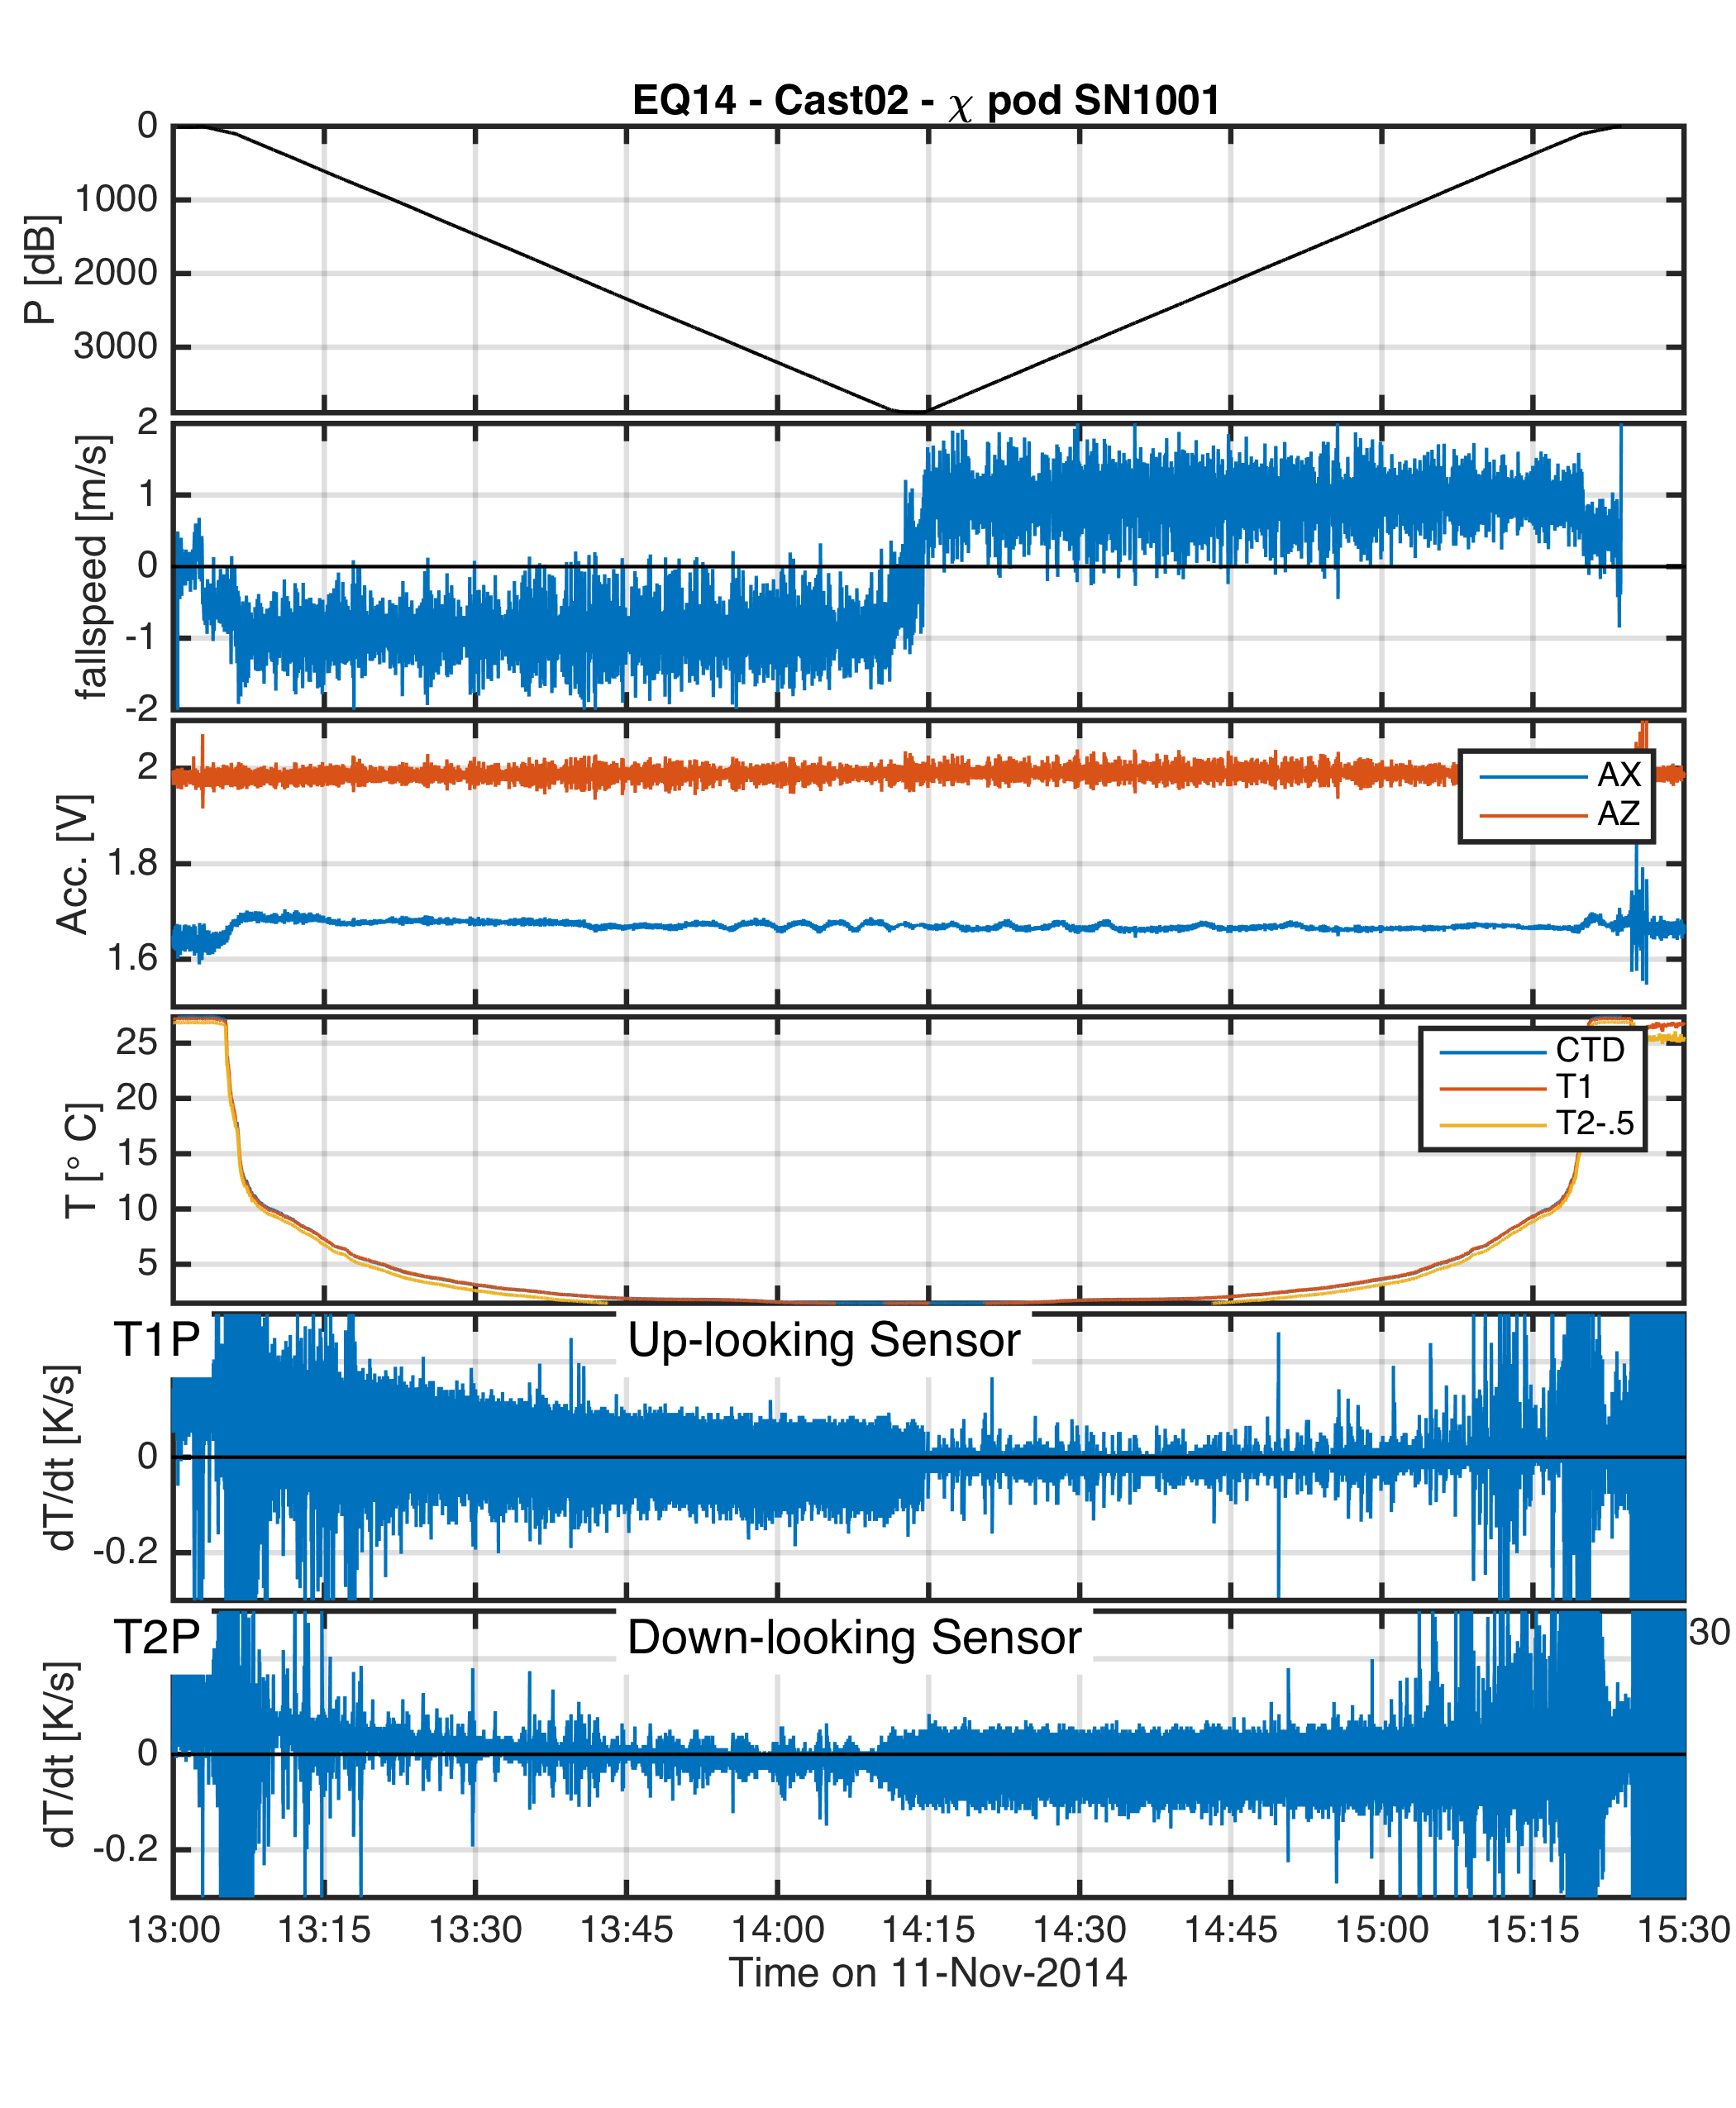
\includegraphics[width=38pc,angle=0]{SN1001_Cast02_Fig5_T_P_dTdz_fspd.png}\\
  \caption{Example timeseries from one CTD cast. a) CTD pressure. b) Fallspeed of CTD ($dp/dz$) .c) Accelerations measured by $\chi$-pod. d) Temperature from CTD and $\chi$-pod (calibrated). e) Temperature derivative $dT/dt$ measured by $\chi$-pod sensor 1. f) Temperature derivative $dT/dt$ measured by $\chi$-pod sensor 2.}
  \label{f2}
\end{figure}


\begin{figure}[t]
  \noindent\includegraphics[width=38pc,angle=0]{wind11_specs.png}\\
  \caption{Example temperature gradient spectra from EQ14. Solid blue and black lines show the observed spectra, before and after a response correction was applied. Dashed lines show the theoretical Kraichnan spectra for the $\chi$pod estimates. Purple line is Kraichnan spectra for chameleon $\chi$ and $\epsilon$. Vertical dashed line indicates the maximum wavenumber used in the $\chi$pod calculation.}
  \label{specexamp}
\end{figure}


% PlotHistKbRatio.m
\begin{figure}[t]
  \noindent\includegraphics[width=38pc,angle=0]{Hist_kbrat.png}\\
  \caption{Histogram of the ratio of the maximum observed wavenumber $k_{max}$ to the Batchelor wavenumber $k_b$ for all profiles in EQ14.}
  \label{histkbrat}
\end{figure}



% Plot_chiProc_vs_actual_EQ14
\begin{figure}[t]
  \noindent\includegraphics[width=38pc,angle=0]{EQ14_chiVsTrue_chi_zsm10m_fmax15Hz_respcorr1_fc_10hz_gamma20.png}\\
  \caption{Depth-time plots of $\chi$ from both methods for EQ14 data.}
  \label{eq14_eps_pcolor}
\end{figure}


\begin{figure}[t]
  \noindent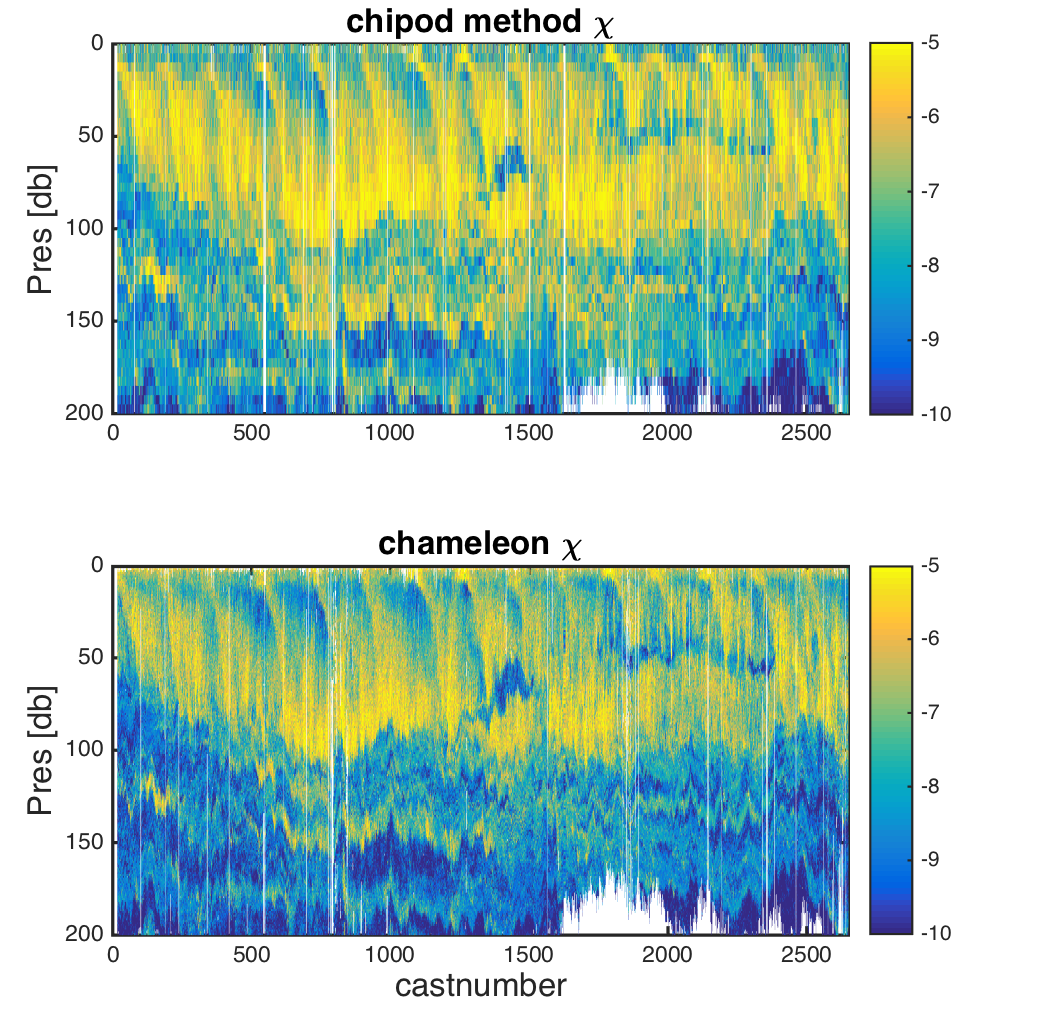
\includegraphics[width=38pc,angle=0]{EQ08_chiVsTrue_chi_zsm10m_fmax10Hz_respcorr1_gamma20.png}\\
  \caption{Depth-time plots of $\chi$ from both methods for EQ08 data.}
  \label{eq08_eps_pcolor}
\end{figure}


\begin{figure}[t]
  \noindent\includegraphics[width=38pc,angle=0]{EQ14_2dhist_chi_zsm10m_fmax15Hz_respcorr1_fc_10hz_gamma20.png}\\
  \caption{2D histogram of $\chi$ from chameleon (x-axis) and chipod method (y-axes). Each panel uses a different value of fmax.}
  \label{eq14_chi_2dhist}
\end{figure}


\begin{figure}[t]
  \noindent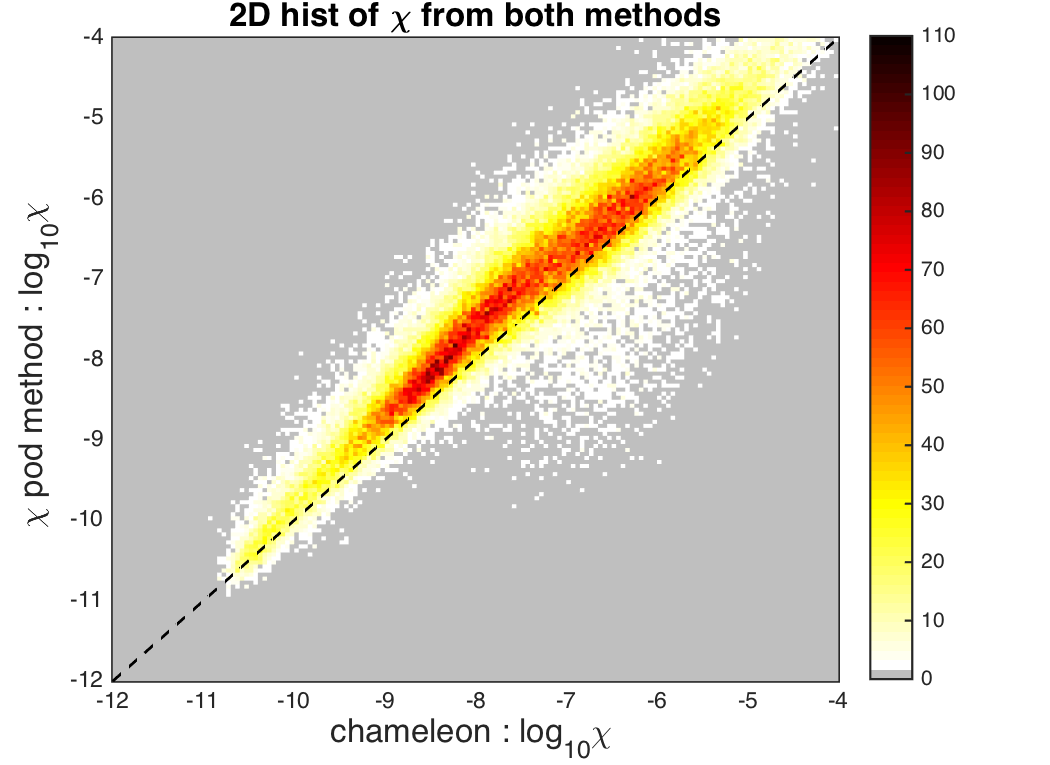
\includegraphics[width=38pc,angle=0]{EQ08_2dhist_chi_zsm10m_fmax10Hz_respcorr1_gamma20.png}\\
  \caption{EQ08: 2D histogram of $\chi$ from chameleon (x-axis) and chipod method (y-axes). Each panel uses a different value of fmax.}
  \label{eq08_chi_2dhist}
\end{figure}


\begin{figure}[t]
  \noindent\includegraphics[width=38pc,angle=0]{EQ14_ctdChipod_vs_chamMean_chi_scatter_zsm20_fmax20.png}\\
  \caption{Scatter plot of $\chi$ from CTD-$\chi$pod profiles versus the mean of bracketing chameleon profiles. Black dashed line shows 1:1, red are $\pm$ 10 X. **replace with histogram of ratios, or combine into one figure?**}
  \label{eq14_cdtChi_vs_cham}
\end{figure}


\begin{figure}[t]
  \noindent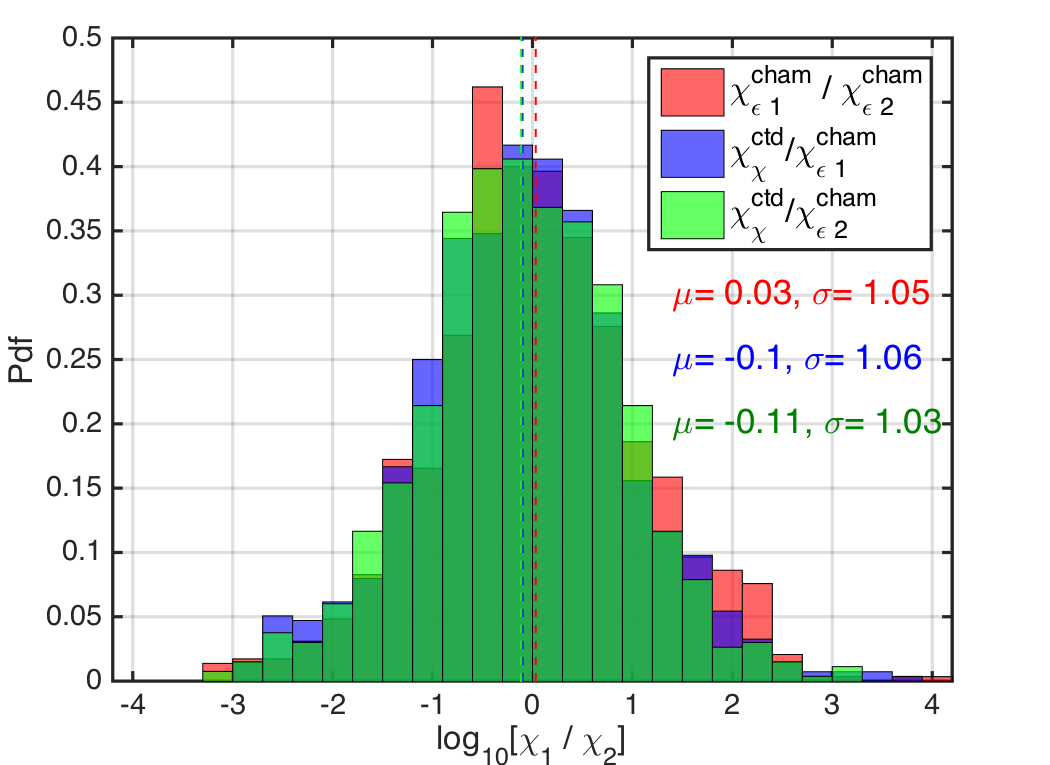
\includegraphics[width=38pc,angle=0]{EQ14_CtdChipod_hist_chi_ratios.png}\\
  \caption{Histogram of $log_{10}$ of the ratio of $\chi$ for nearby casts. One line is for CTD-$\chi$pod profiles versus the bracketing chameleon profiles. Another line is for the before vs. after chameleon profiles. *Note bias is small/zero, and the variability (spread) between CTD/cham is similar to the natural variability between cham profiles.*}
  \label{eq14_cdtChi_vs_cham_hist}
\end{figure}


%\begin{figure}[t]
%  \noindent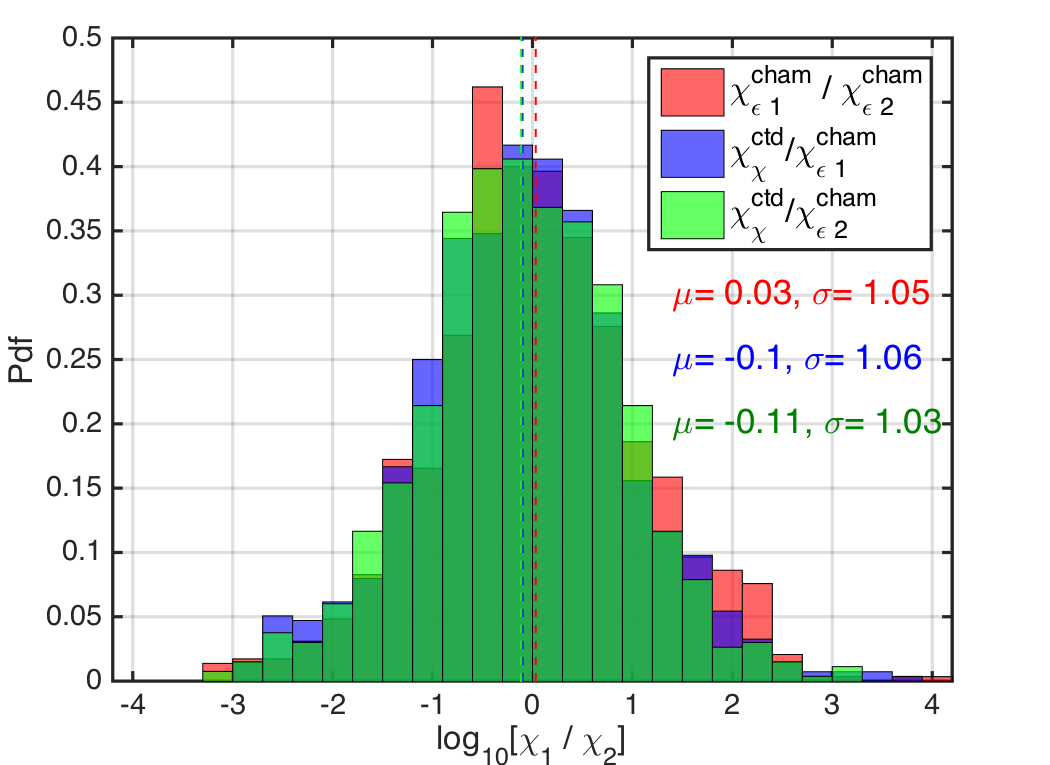
\includegraphics[width=38pc,angle=0]{EQ14_CtdChipod_hist_chi_ratios.png}\\
%  \caption{Histogram of the ratio of $\chi$ from CTD-$\chi$pod profiles to the mean of bracketing chameleon profiles. }
%  \label{}
%\end{figure}




\begin{figure}[t]
  \noindent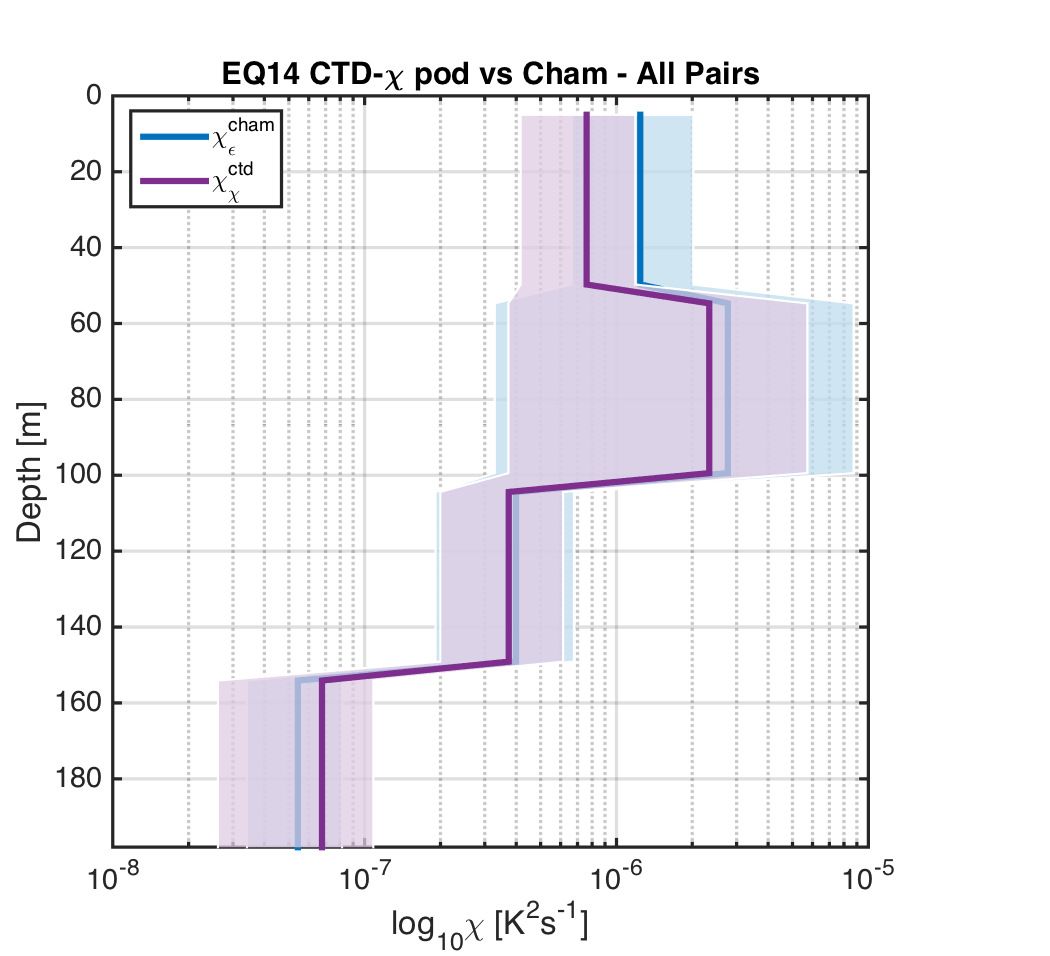
\includegraphics[width=38pc,angle=0]{EQ14_chi_cham_meanProf_all.png}\\
  \caption{Time mean of $\chi$ for all CTD-$\chi$pod - chameleon cast pairs, with 95\% bootstrap confidence intervals.}
  \label{ctd_cham_chi_boot_all}
\end{figure}

\begin{figure}[t]
  \noindent\includegraphics[width=38pc,angle=0]{P16N_BothLegs_Transect_Combined.png}\\
  \caption{Example chipod data from P16N. *need to clean up*}
  \label{}
\end{figure}


\begin{figure}[t]
  \noindent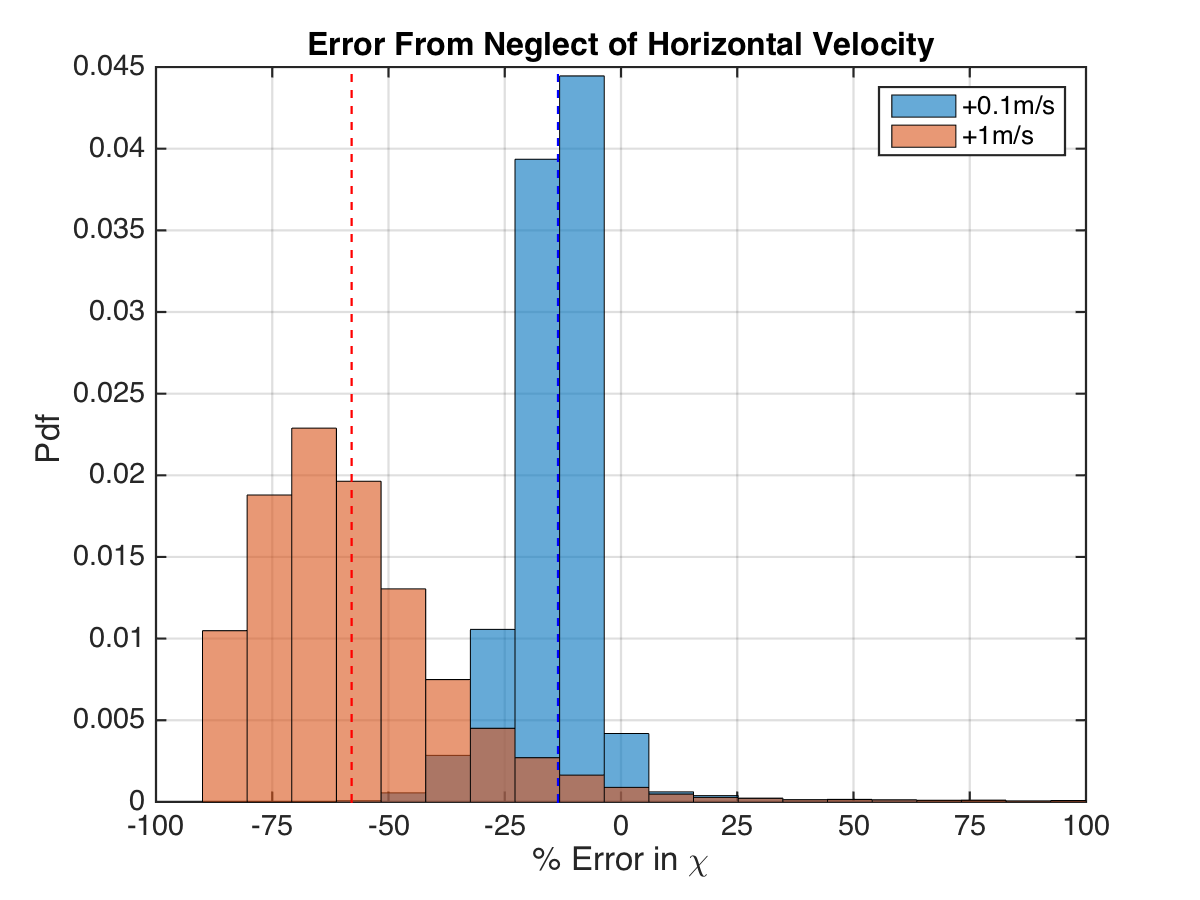
\includegraphics[width=38pc,angle=0]{Hist_perr_fspdvary.png}\\
  \caption{Histogram of \% error for $\chi$ computed with constant $\pm$ fspd added.}
  \label{FspdSensHist}
\end{figure}



%
%%~~ F1
%\begin{figure}[t]
%  \noindent\includegraphics[width=38pc,angle=0]{F1_sADCP_CTDandVMP_upper.png}\\
%  \caption{Data from station `F1', which consisted of 30 hours of LADCP/CTD followed by about 8 hours of VMP profiling. Note that only upper 800m are shown. a) Barotropic tidal velocity from TPXO. b) Zonal velocity measured by LADCP (up to 0600 on Sept. 9), and shipboard ADCP (after 0600 on Sept. 9). c) Same as b, but for meridional velocity. d) Temperature measured by CTD and VMP. e) Turbulent dissipation rate $\epsilon$ measured by $chi$-pod and VMP.}
%  \label{f3}
%\end{figure}
%
%\begin{figure}[t]
%  \noindent\includegraphics[width=38pc,angle=0]{F1_EpsProfilesAvg_BinBoot.png}\\
%  \caption{Time-average profiles of $\epsilon$ at station F1, from $\chi$-pod and VMP profiles. Data are averaged in 100m depth bins. Shading indicates 95\% confidence intervals from bootstrapping.}
%  \label{f4}
%\end{figure}
%
%
%%~~ N1a
%\begin{figure}[t]
%  \noindent\includegraphics[width=38pc,angle=0]{N1a_sADCP_CTDandVMP_upper.png}\\
%  \caption{Data from station `N1a' . Note only upper 1000m are shown. a) Barotropic tidal velocity from TPXO. b) Zonal velocity measured by LADCP (right), and shipboard ADCP (left). c) Same as b, but for meridional velocity. d) Temperature measured by CTD and VMP. e) Turbulent dissipation rate $\epsilon$ measured by $chi$-pod and VMP.}
%  \label{n1a1}
%\end{figure}
%
%\begin{figure}[t]
%  \noindent\includegraphics[width=38pc,angle=0]{N1a_EpsProfilesAvg_BinBoot.png}\\
%  \caption{Time-average profiles of $\epsilon$ at station N1a, from $\chi$-pod and VMP profiles. Data are averaged in 100m depth bins. Shading indicates 95\% confidence intervals from bootstrapping.}
%  \label{n1a2}
%\end{figure}
%
%
%%~~ S4
%\begin{figure}[t]
%  \noindent\includegraphics[width=38pc,angle=0]{S4_sADCP_CTDandVMP_upper.png}\\
%  \caption{Data from station `S4' . Note only upper 600m are shown. a) Barotropic tidal velocity from TPXO. b) Zonal velocity measured by LADCP (up to 0600 on Aug. 19), and shipboard ADCP (after 0600 on Aug. 19). c) Same as b, but for meridional velocity. d) Temperature measured by CTD and VMP. e) Turbulent dissipation rate $\epsilon$ measured by $chi$-pod and VMP.}
%  \label{s41}
%\end{figure}
%
%\begin{figure}[t]
%  \noindent\includegraphics[width=38pc,angle=0]{S4_EpsProfilesAvg_BinBoot.png}\\
%  \caption{Time-average profiles of $\epsilon$ at station S4, from $\chi$-pod and VMP profiles. Data are averaged in 100m depth bins. Shading indicates 95\% confidence intervals from bootstrapping.}
%  \label{s42}
%\end{figure}


% All stations chi vs OT
% Plot_OT_chi_IWISE10_OneFig.m
%\begin{figure}[t]
%  \noindent\includegraphics[width=38pc,angle=0]{AllStations_EpsProfilesAvg_iwise10.png}\\
%  \caption{Time-average profiles of $\epsilon$ at  from $\chi$-pod and overturns. Data are averaged in xxm depth bins. Shading indicates 95\% confidence intervals from bootstrapping? Dashed black line shows estimated noise level for $\epsilon_{OT}$ using equation (7) in \cite{galbraithkelley96}.** add noise levels to plots. For OT this is just proportional to N2 and CTD noise. For chi need to figure out.}
%  \label{allprofiles}
%\end{figure}

\end{document}